\chapter{Sprint 0: Plannification du projet}
\etocsettocstyle{\section*{Sommaire}}{}
\localtableofcontents
\section{Introduction}
\noindent
Dans ce chapitre, on va présenter la premiére phase de la méthode SCRUM, qui est le Sprint 0, qui ce commence par l'identification des besoins. Par la suite, nous faisons une analyse globale de notre projet en identifiant les acteurs et ensuite le Diagramme de Cas D'Utilisation globale. De plus, nous planifions le reste des sprints de notre projet. Puis, en va présnter l'architecture du systéme pour laquelle nous avons opté. Et enfin, en va présenter les outils de développement utilisés pour réaliser ce projet.

\section{Identification des besoins}
\subsection{Les besoins fonctionnels}
\noindent
Les besoins fonctionnels sont les fonctionnalités que le systéme doit livrer aux utilisateurs.
L’outil n’est considéré comme opérationnel que si sa disponibilité fonctionnelle est garantie.
Dans le cas du notre systéme, ces besoins se concentrent sur:

\begin{itemize}
    \item \small\textbf{Vitesse de recherche: } {Améliorer les vitesses de recherche au maximum afin de renvoyer des résultats précis au client.}
    
    \item \small\textbf{Recherche en Français: } {Permettre le client a rechercher les produits dans la langage Française.}

    \item \small\textbf{Recherche en Arabe Tunisienne: } {Permettre le client a rechercher les produits dans la langage Arabe Tunisienne.}

    \item \small\textbf{Recherche en Arabe Traditionnel: } {Permettre le client a rechercher les produits dans la langage Arabe Classique.}
    
    \item \small\textbf{Suggestion des produits: } {Si le produit recherché par le client n'existe pas, le système tentera de suggérer des produits similaires en prenant le contexte du terme de recherche.}
\end{itemize}

\newpage
\subsection{Les besoins non fonctionnels}
\noindent
Les exigences non fonctionnels décrivent les objectifs liés aux performances du systéme et d'autres aspects cruciaux du système qui ne sont pas directement liés à ses fonctionnalités spécifiques. Ils définissent les critères de qualité que le système doit respecter pour répondre aux attentes des utilisateurs. Notre systéme doit repondre aux exigences non fonctionnels suivantes:

\begin{itemize}
    \item \small\textbf{La Fiabilité: } L'application doit être fonctionnelle sans détection des erreurs afin de satisfaire les besoins de client.

    \item \small\textbf{La Sécurité: } Vu que l'application contient des données confidentielles, tous l'accés des produits doivent être protégées par un privilege d'accées.

     \item \small\textbf{La Disponibilité: } Les services offerts par notre application sont disponibles pendant les 24
     heures et durant toute la semaine.

     \item \small\textbf{La Performance: } L'application doit être rapide et robuste (Vitesse de réponse rapide et précision des résultats lors du recherche des produits dans les langues différents).
\end{itemize}

\newpage
\section{Diagramme de cas d’utilisation global}
\subsection{Introduction}
\noindent
Dans cette partie, on va présenter les besoins de notre systéme de façon formelle à l'aide du diagramme de cas d'utilisation du langage de modélisation UML. D'abord nous identifions les acteurs qui intéragissent avec notre systéme, qui sont:

\noindent
\small\textbf{Le Visiteur: } C'est le personne qui va accéder à notre systéme pour rechercher le(s) produit(s) dans notre systéme.

\noindent
\small\textbf{Le Client: } C'est aussi le personne qui va accéder à notre systéme pour rechercher le(s) produit(s) de ses besoins. 

\noindent
\small\textbf{L'Admin: } C'est le personne qui va accéder à notre systéme pour rechercher le(s) produit(s) dans notre systéme et modifier les paramétres de son recherche. 

\begin{figure}[H]
\centering
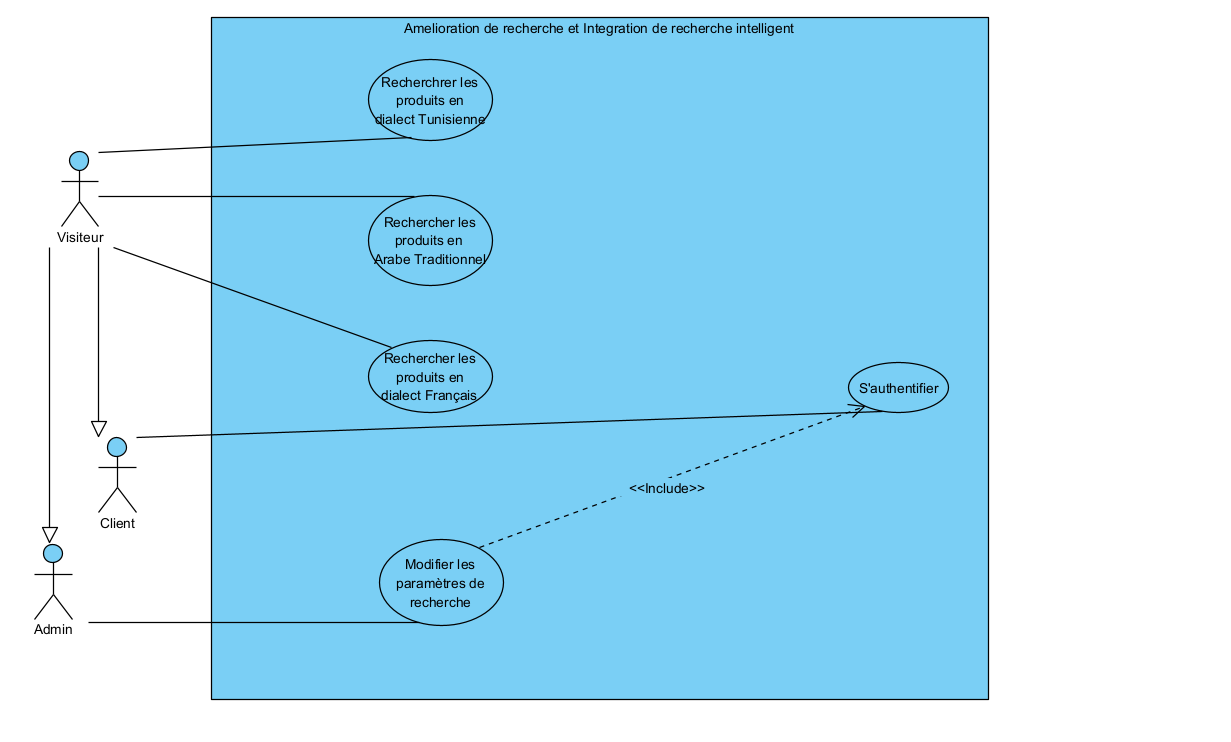
\includegraphics[width=1\textwidth]{logos/CU_global.png}
\caption{Présentation de Diagramme de Cas D'Utilisation global}
\label{fig:diagcuglobal}
\end{figure}
\section{Backlog De Produit}
\noindent
\large
Le backlog de produit est une liste de fonctionnalités à réaliser. Ces fonctionalités sont exprimées sous formes des besoins et sont priorisées par le Product Owner ce qui permet d'établir un ordre de réalisation à respecter. \\
Notre backlog est composé de trois colonnes: \\
\textbf{ID: } C'est l'identifiant du scénario \\
\textbf{Fonctionnalité: } Permet de mieux ordonner les scénarios. \\
\textbf{Scénario: } Comporte la description des scénarios suivant le forme << En tant que ... Je veux >> \\

\begin{table}[H]
\centering
\begin{tabular}{|c|c|p{10cm}|}
\hline
\rowcolor{blue!20}
\textbf{ID} & \textbf{Fonctionnalité} & \textbf{Scénario} \\ \hline
1 & Recherche en Arabe Tunisienne  & En tant qu'un client, je veux rechercher un ou plusieurs produits dans la langue Tunisienne. \\ \hline
2 & Recherche en Arabe Classique & En tant qu'un client, je veux rechercher un ou plusieurs produits en Arabe Classique. \\ \hline
3 & Recherche en Français & En tant qu'un client, je veux rechercher un ou plusieurs produits en Français. \\ \hline
4 & Vitesse de recherche & En tant qu'un client, je veux avoir une vitesse de recherche rapide. \\ \hline
5 & Suggestion des produits & En tant qu'un client, si le produit que je cherche n'existe pas, je veux avoir des suggestions des produits similaires. \\ \hline
\end{tabular}
\caption{Table des fonctionnalités et scénarios.}
\end{table}
\section{La Plannification De Release}
\noindent
Une fois que le Product Owner a fini de construire le Product Backlog, l'équipe SCRUM et l'environnement technique du projet est bien mis en œuvre, et tous le membres du projet sont plannifiés le sprint ensemble aussi que les fonctionnalités à développer pour chaque Sprint, la durée de la prévision de chaque sprint est estimée à quatre semaines.
\section{Architecture du systéme}
\noindent
Il est indispensable à la conception de tout systéme informatique de choisir le modéle d'architecture adéquat et pourra assurer le bon fonctionnement, une meilleure performance, ainsi que la scalabilité, la fiabilité et trés important, la productivité de développement. \\
C'est pour cette raison, qu'on a opté pour l'architecture MVC avec des microservices (Modèle, Vue, Contrôleur, Modèle IA, et Elasticsearch) comme l'architecture global du projet, et le modèle << Clean Architecture >>, dans le backend, qui seront trés pratique pour gérer les intéractions entre les différents composants de notre application. Nous décrirons ces architectures dans les prochaines sections.

\subsection{Architecture "MVC Avec Microservices"}
\noindent
Le modèle MVC permet de bien organiser son code source. Il va nous aider à savoir quels fichiers créer, mais surtout à définir leur rôle. Le but de MVC est justement de séparer la logique du code en trois parties que l'on retrouve dans des fichiers distincts.

\noindent
{\small\textbf{\textit{Modèle}}}\mbox{}\\
Cette partie gère ce qu'on appelle la logique métier de notre site. Elle comprend notamment la gestion des données qui sont stockées, mais aussi tout le code qui prend des décisions autour de ces données. Son objectif est de fournir une interface d'action la plus simple possible au contrôleur. On y trouve donc entre autres des algorithmes complexes et des requêtes SQL, et Elasticsearch dans notre cas.

\noindent
{\small\textbf{\textit{Vue}}}\mbox{}\\
Cette partie se concentre sur l'affichage. Elle ne fait presque aucun calcul et se contente de récupérer des variables pour savoir ce qu'elle doit afficher. On y trouve essentiellement du code HTML mais aussi quelques boucles et conditions Javascript très simples, pour afficher par exemple une liste de messages. Il est développé avec React et Typescript.

\noindent
{\small\textbf{\textit{Contrôleur}}}\mbox{}\\
Cette partie gère les échanges avec l'utilisateur. C'est en quelque sorte l'intermédiaire entre l'utilisateur, le modèle et la vue. Le contrôleur va recevoir des requêtes de l'utilisateur. Pour chacune, il va demander au modèle d'effectuer certaines actions (demander les produits en fonction d'un mot-clé de recherche) et de lui renvoyer les résultats (la liste des produits). Puis il va adapter ce résultat et le donner à la vue. Enfin, il va renvoyer la nouvelle page HTML, générée par la vue, à l'utilisateur. Il est implémenté avec ASP .NET Core et C\# et utilise des requêtes SQL et Elasticsearch pour manipuler les donnèes.

\noindent
{\small\textbf{\textit{Modèle IA}}}\mbox{}\\
Notre modèle IA a une et une seule responsabilité, qui est de faire l'encodage de la requête de l'utilisateur qui est envoyé au contrôleur et retourner le résultat encodé.

\noindent
{\small\textbf{\textit{Elasticseach}}}\mbox{}\\
Elasticsearch agit comme notre base de données de recherche de vecteurs qui contient notre index de produits contenant 2 colonnes de vecteurs recherchables à l'aide du vecteur codé renvoyé par le modèle AI.

\newpage
\noindent
La figure ~\ref{fig:mvc} schématise le rôle de chacun de ces éléments.
\begin{figure}[H]
\centering
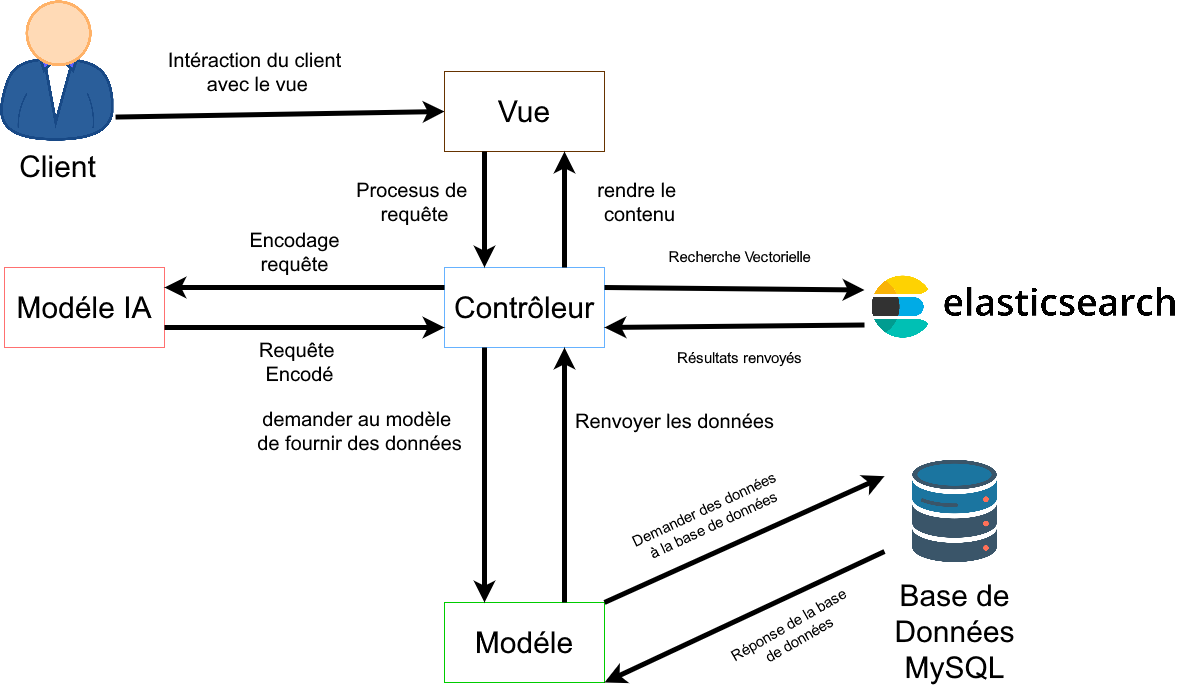
\includegraphics[width=1\textwidth]{logos/mvcavecservice.png}
\caption{L'architecture MVC avec microservices}
\label{fig:mvc}
\end{figure}

\noindent
Il est important de bien comprendre comment ces éléments s'agencent et communiquent entre eux. La figure ~\ref{fig:mvcechange} montre cette communication.

\begin{figure}[H]
\centering
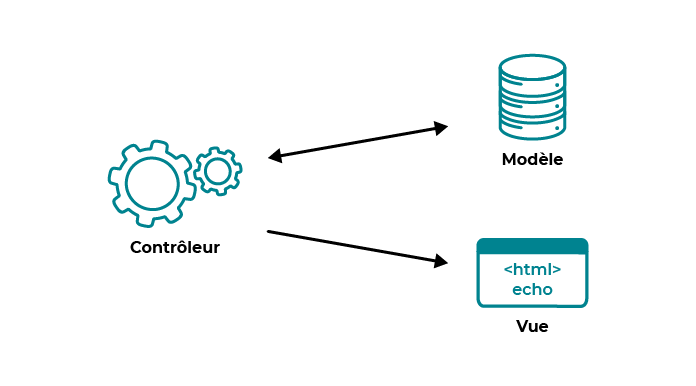
\includegraphics[width=1\textwidth]{logos/mvcechange.png}
\caption{Échange d'informations entre les éléments MVC}
\label{fig:mvcechange}
\end{figure}

\subsection{Architecture "Clean Architecture"}
\noindent
"Clean Architecture" est un modèle architectural introduit par Robert C. Martin, également connu sous le nom d'Oncle Bob. Il favorise une séparation claire des préoccupations en divisant l'application en couches concentriques, chaque couche ayant ses responsabilités et ses dépendances. Le principe fondamental derrière l'architecture propre est la règle de dépendance, qui stipule que les dépendances doivent toujours pointer vers l'intérieur vers les couches les plus stables et abstraites, plutôt que vers l'extérieur vers des couches plus concrètes et volatiles. 

\noindent
Cette architecture se compose généralement des couches suivantes: \\

\begin{itemize}
    \small\item \textbf{La couche Presentation: } Cette couche est responsable de la gestion des interactions des utilisateurs et de la fourniture des données à l'interface utilisateur. Dans notre context d'une API Web .NET Core, cette couche comprend les contrôleurs et autres composants qui gèrent les requêtes et les réponses HTTP.

    \small\item \textbf{La couche Application: } La couche Application contient la logique métier et les cas d’utilisation de l’application. Il agit comme intermédiaire entre la couche présentation et la couche domaine. Cette couche est indépendante de tout problème spécifique d’interface utilisateur ou d’infrastructure.
    \small\item \textbf{La couche Domain: } La couche Domain représente le noyau de l’application, encapsulant les règles métier, les entités, les interfaces (Orienté Objet) des repositories des bases de donnés et la logique spécifique au domaine. Il doit être indépendant de la technologie et ne contenir aucune dépendance vis-à-vis de frameworks ou de bibliothèques externes.

    \small\item \textbf{La couche Infrastructure: } La couche infrastructure traite des problèmes externes tels que les bases de données, les services externes et les frameworks. Il contient des implémentations d'interfaces définies dans la couche application et interagit avec des ressources externes.
\end{itemize}

\noindent
La figure Figure~\ref{fig:architecture} reprèsente les couches de << Clean Architecture >>

\begin{figure}[H]
\centering
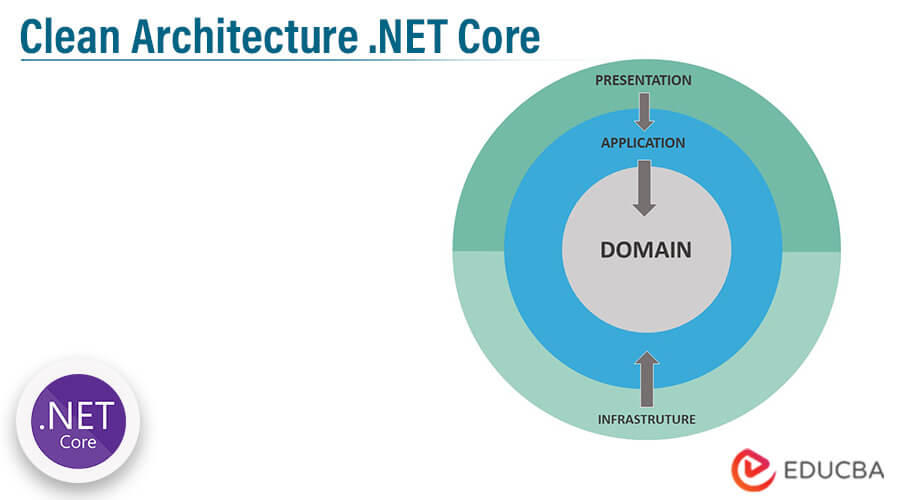
\includegraphics[width=1\textwidth]{logos/clean_architecture.png}
\caption{Architecture "Clean Architecture" dans ASP. NET Core}
\label{fig:architecture}
\end{figure}

\noindent
Les avantages de l’utilisation de  << Clean Architecture >> :

\begin{itemize}[label={---}]
    \item \small\textbf{Vitesse d'implementation: } La mise en œuvre immédiate vous permet d'implémenter cette architecture avec n'importe quel langage de programmation.

    \item \small\textbf{Les couches de Domain et Application comme noyau du système}: Les couches Domain et Application sont toujours au centre de la conception et sont connus comme le cœur du système, c'est pourquoi le cœur du système ne dépend pas de systèmes externes. 

    \item \small\textbf{Indépendence des systémes externes: } Cette architecture permet de changer de système externe sans affecter le cœur du système.

    \item \small\textbf{Testabilité améliorée du code: } Dans un environnement qui depends hautement des tests(unitaires et d'intégration), vous pouvez tester votre code rapidement et facilement.    

    \item \small\textbf{Création de produits scalables, robustes et de haute qualité: } Vous pouvez vitement créer un systéme bien performant, organisé, testable, scalable, et robuste.
\end{itemize}
\noindent
\section{L'environnement de développement et choix techniques: }

\subsection{Introduction}
\noindent
Le développement de notre projet nécessite un ordinateur avec des spécifications puissantes en raison de choses telles que le développement de C\# dans Visual Studio, le lancement des containers Docker, le lancement et le stockage de données dans Elasticsearch, l'importation et l'utilisation de notre modèle Sentence-Transformers, et surtout l'exécution de la recherche vectorielle. C'est pour cette raison que nous disposons d'ordinateurs avec les spécifications mentionnées dans la section  de l'environnement matériel ci-dessous. \\
\citetitle{elastic:hardwarespecifications} (\cite{elastic:hardwarespecifications})

\subsection{L'environnement matériel}
\noindent
Dans la table~\ref{tab:compspec} nous mentionnons les spécifications des ordinateurs utilisés pour le développement de notre application: 

\begin{table}[H]
\centering
\begin{tabular}{|c|c|c|c|}
\hline
\rowcolor{blue!20}
\textbf{Processeur} & \textbf{Mémoire} & \textbf{Disque dur} & \textbf{Système d'exploitation} \\
\hline
11th Gen Intel Core i7 @ 2.304GHz & 32Go & 1.5To SSD & Windows 11-64bits \\
\hline
9th Gen Intel Core i7 @ 1.8GHz & 32Go & 1To SSD 1To HDD & Windows 10-64bits \\
\hline
\end{tabular}
\caption{Spécifications des ordinateurs utilisés}
\label{tab:compspec}
\end{table}

\newpage
\subsection{L'environnement logiciel}
\noindent
{\small\textbf{\textit{Visual Studio}}}\mbox{}\\
Visual Studio est un environnement de développement intégré (IDE) créé par Microsoft. Il est principalement utilisé pour le développement de logiciels, notamment pour les langages de programmation tels que C\#, C++. Pour C\# il offre beacoup des outils qui aide et accélére et améliore l'expérience de développement comme une complétion automatique intelligente, création des classes/interfaces intelligente et un débogeur puissant pour détecter et résoudre les erreurs. La figure ~\ref{fig:vs} présente le logo de Visual Studio.

\begin{figure}[H]
\centering

\includegraphics[width=0.3\textwidth]{logos/vs.png}
\caption{Logo officiel du logiciel Visual Studio}
\label{fig:vs}
\end{figure}

\noindent
{\small\textbf{\textit{Visual Studio Code}}}\mbox{}\\
Visual Studio Code (VS Code) est un éditeur de code source gratuit et open source développé par Microsoft connu par sa légèreté, rapidité et personnalisation à travers les extensions qu'il fournit pour une diversité des langages de programmation.
Il fournit beaucoup de choses qu'un IDE fait comme la coloration syntaxique, la complétion automatique, et le déboggage, et la gestion de versions intégré. La figure ~\ref{fig:vsc} présente le logo de Visual Studio Code.
\begin{figure}[H]
\centering

\includegraphics[width=0.3\textwidth]{logos/vsc.png}
\caption{Logo officiel du logiciel Visual Studio Code}
\label{fig:vsc}
\end{figure}

\noindent
{\small\textbf{\textit{C\#}}}\mbox{}\\
C\# (prononcé "C sharp") est un langage de programmation de haut niveau, orienté objet, développé par Microsoft dans le cadre de sa plateforme .NET. Lancé en 2000, C\# a été conçu pour être simple, moderne, sûr et évolutif. C\# est utilisé pour le développement  d'une variété des applications, nottament des applications backend et des REST API web avec ASP .NET Core. La figure ~\ref{fig:cs} présente le logo de C\#.
\begin{figure}[H]
\centering

\includegraphics[width=0.3\textwidth]{logos/csharp.png}
\caption{Logo officiel du langage de programmation C\#}
\label{fig:cs}
\end{figure}

\noindent
{\small\textbf{\textit{ASP .NET Core}}}\mbox{}\\
ASP.NET Core est un framework open source développé par Microsoft pour la création d'applications web modernes. Il constitue la prochaine évolution de la plateforme ASP.NET, offrant une architecture modulaire, légère et hautement performante. Il offre une large flexibilité et une modularité au développeurs, il prend en charge principalement le développement des APIs web RESTful qui peuvent être déployé sur Windows, Linux et MacOS. Il offre une variété des fonctionallités comme le traitement asynchrone des requêtes, le middleware et le pipeline de requêtes personnalisable.
la figure ~\ref{fig:netcore} présente le logo de ASP .NET Core.
\begin{figure}[H]
\centering

\includegraphics[width=0.3\textwidth]{logos/dotnetcore.png}
\caption{Logo officiel du framework ASP .NET Core}
\label{fig:netcore}
\end{figure}

\noindent
{\small\textbf{\textit{Python}}}\mbox{}\\
Python est un langage de programmation interprété, de haut niveau, polyvalent puisqu'il est utilisé dans plusieurs domaines notamment l'analyse de données et le machine learning (avec des bibliothèques telles que NumPy, Pandas, et PyTorch). La figure ~\ref{fig:py} présente le logo de Python.
\begin{figure}[H]
\centering

\includegraphics[width=0.3\textwidth]{logos/pypng.png}
\caption{Logo officiel du langage de programmation Python}
\label{fig:py}
\end{figure}

\noindent
{\small\textbf{\textit{Jupyter Notebook}}}\mbox{}\\
Jupyter Notebook est une application web open source qui permet de créer et de partager des documents interactifs contenant du code qui sont composés des cellules de code qui peuvent être exécuté individuellement, et facilement partagé à travers des differents sites comme Kaggle, Google Collab. La figure ~\ref{fig:jupyter} présente le logo de Jupyter.
\begin{figure}[H]
\centering

\includegraphics[width=0.3\textwidth]{logos/jupyter.png}
\caption{Logo officiel du framework Jupyter}
\label{fig:jupyter}
\end{figure}


\noindent
{\small\textbf{\textit{Flask}}}\mbox{}\\
Flask est un framework Python trés minimalistique pour développer des REST APIs en Python. Il est très facile de configurer et de faire fonctionner une API. Et pour cette raison, nous l'avons utilisé pour exposer un point de terminaison d'API REST unique afin d'exposer notre modèle Sentence-Transformers. La figure ~\ref{fig:flask} présente le logo de Flask.
\begin{figure}[H]
\centering
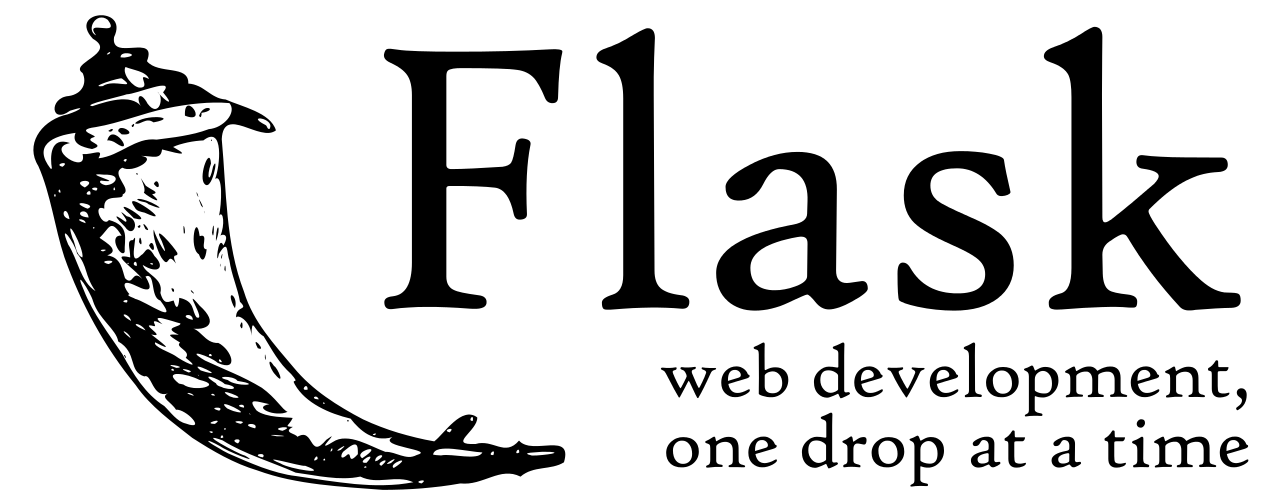
\includegraphics[width=0.3\textwidth]{logos/flask.png}
\caption{Logo officiel du framework Flask}
\label{fig:flask}
\end{figure}


\noindent
{\small\textbf{\textit{React}}}\mbox{}\\
React est un framework Javascript gratuit et open-source développé et maintenu par méta(anciennement sous le nom Facebook) en 2013 utilisée principalement pour le développement des interfaces utilisateurs web complexes à travers des "components", ou composants en Français. La figure ~\ref{fig:react} présente le logo de React.
\begin{figure}[H]
\centering

\includegraphics[width=0.3\textwidth]{logos/react.png}
\caption{Logo officiel du bibilothéque React}
\label{fig:react}
\end{figure}

\noindent
{\small\textbf{\textit{Typescript}}}\mbox{}\\
Typescript est un langage de programmation gratuit et open-source développé et maintenu par Microsoft principalement pour améliorer l'expérience de développement pour les développeurs Javascript en fournisaant des types statiques, des erreurs directement dans l'éditeur de code, et support totale pour la programmation Orienté Objet. La figure ~\ref{fig:typescript} présente le logo de Typescript.
\begin{figure}[H]
\centering

\includegraphics[width=0.3\textwidth]{logos/typescript.png}
\caption{Logo officiel du langage Typescript}
\label{fig:typescript}
\end{figure}

\noindent
{\small\textbf{\textit{Docker}}}\mbox{}\\
Docker est une plateforme open source qui permet de développer, de déployer et d'exécuter des applications de manière efficace en utilisant des conteneurs logiciels. Les conteneurs sont des unités d'exécution légères et autonomes qui encapsulent une application et tous ses composants, y compris les bibliothèques, la version de langages de programmation utilisè(s), les ports exposès... 
la figure ~\ref{fig:docker} prèsente le logo de Docker.
\begin{figure}[H]
\centering

\includegraphics[width=0.3\textwidth]{logos/docker.png}
\caption{Logo officiel du Docker}
\label{fig:docker}
\end{figure}

\noindent
{\small\textbf{\textit{Elasticsearch}}}\mbox{}\\
Elasticsearch est un outil d'analyse de donnèes distribuès open source et hautement èvolutif. Il est conçu pour stocker, rechercher et analyser et rechercher de grands volumes de données de manière rapide et efficace en utilisant des diffèrents mèthodes comme Knn Search.
Il utilise une structure de données de type index inversé pour indexer et rechercher rapidement des documents. Il prend en charge une variété de types de données, notamment le texte, les nombres, les dates, et les vecteurs par exemple le type dense vector.
La figure ~\ref{fig:elasticsearch} prèsente le logo d'Elasticsearch.
\begin{figure}[H]
\centering

\includegraphics[width=0.3\textwidth]{logos/elasticsearch.png}
\caption{Logo officiel d'Elasticsearch}
\label{fig:elasticsearch}
\end{figure}

\noindent
{\small\textbf{\textit{Kibana}}}\mbox{}\\
Kibana est un logiciel de visualisation de données liées à Elasticsearch. Il permet de visualiser et manipuler les indexes stockées dans Elasticsearch ainsi que l'analyse des données de grandes volumes.
La figure ~\ref{fig:kibana} prèsente le logo de Kibana.
\begin{figure}[H]
\centering

\includegraphics[width=0.3\textwidth]{logos/kibana.png}
\caption{Logo officiel du Kibana}
\label{fig:kibana}
\end{figure}

\noindent
{\small\textbf{\textit{Postman}}}\mbox{}\\
Postman est une plateforme API qui permet de construire, tester et utiliser des APIs en simplifiant et organisant les étapes nécessaires comme la création des workspaces, qui permet un utilisateur de regrouper plusieurs endpoints API dans un workspace aussi que le support de différents types de "body". La figure ~\ref{fig:postman} présente le logo de Postman
\begin{figure}[H]
\centering

\includegraphics[width=0.3\textwidth]{logos/postman.png}
\caption{Logo officiel du logiciel Postman}
\label{fig:postman}
\end{figure}

\noindent
{\small\textbf{\textit{Overleaf}}}\mbox{}\\
Overleaf est une plateforme en ligne permettant un éditeur de texte pour LaTeX sans aucun téléchargement de logiciel, aussi connu comme un SaaS (Software as a Service). Il aussi permet l'écriture collaborative des documents comme celui-ci.
La figure ~\ref{fig:overleaf} présente le logo d'Overleaf.
\begin{figure}[H]
\centering

\includegraphics[width=0.3\textwidth]{logos/overleaf.png}
\caption{Logo officiel du Overleaf}
\label{fig:overleaf}
\end{figure}

\noindent
{\small\textbf{\textit{LaTeX}}}\mbox{}\\
LaTeX utilise des commandes de texte pour indiquer comment le document doit être structuré et formaté, plutôt que ce concentrer sur la présentation visuelle. Le document est ensuite compilé en un fichier de format PDF en appliquant les régles typographiques et la mise en page appuyé. La figure ~\ref{fig:latex} présente le logo de LaTeX
\begin{figure}[H]
\centering
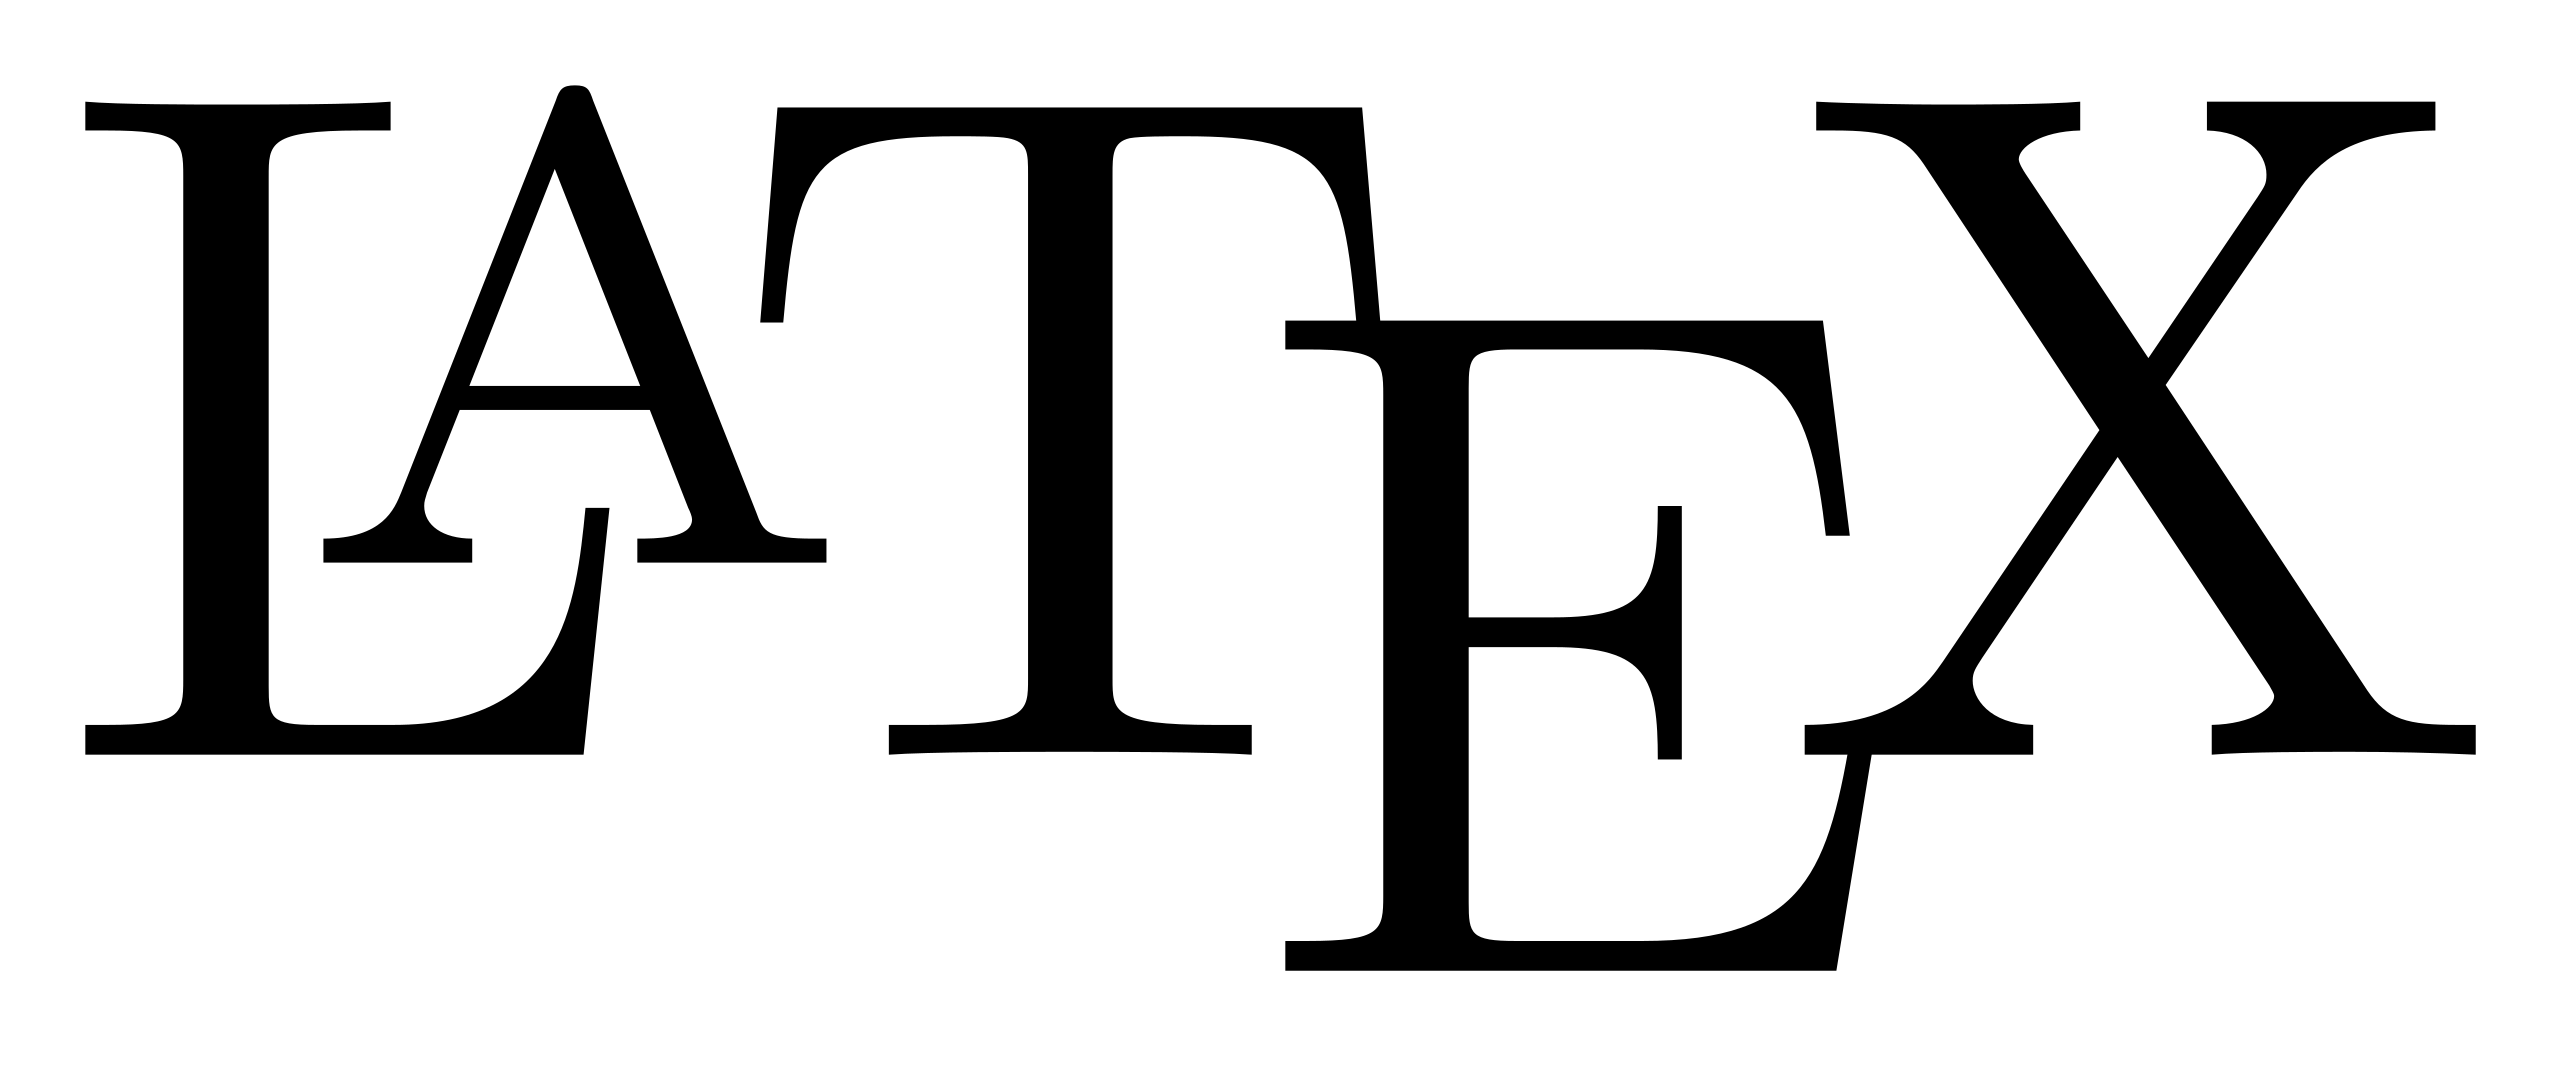
\includegraphics[width=0.3\textwidth]{logos/latex.png}
\caption{Logo officiel du LaTeX}
\label{fig:latex}
\end{figure}

\subsection{Logiciel de modèlisation UML}
\noindent
{\small\textbf{\textit{Visual Paradigm}}}\mbox{}\\
Visual Paradigm est un outil de conception de diagrammes UML.Il est capable de prendre en charge de nombreux diagrammes commer-ciaux et techniques comme UML et BPMN. Cette plateform possedéde une interface graphique simplifiant la manipulation de ces fonctionallités comme (Drag \& Drop). La figure ~\ref{fig:vp} présente le logo de Visual Paradigm.

\begin{figure}[H]
\centering

\includegraphics[width=0.3\textwidth]{logos/vp.png}
\caption{Logo officiel du Visual Paradigm}
\label{fig:vp}
\end{figure}


\section{Conclusion}
\noindent
Dans cette section, nous avons préparé notre plan de travail. Nous avons capturé les besoins fonctionnels et non fonctionnels de notre applcation et nous avons fixé nos choix techniques .
Dans le chapitre qui suit nous allons présenter le premier sprint. 